%%%%%%%%%%%%%%%%%%%%%%%%%%%%%%%%%%%%%%%%%%%%%%%%%%%%%%%%%%%%%%%%%%%%
%%%%%%%%%%%%%%%%%%%%%%%%%%%%%%%%%%%%%%%%%%%%%%%%%%%%%%%%%%%%%%%%%%%%
% BSS Seminar Paper Template 
% © Fynn Lohre 
%
% In case of any questions, reach out to: VARFynn@gmail.com.
%
%%%%%%%%%%%%%%%%%%%%%%%%%%%%%%%%%%%%%%%%%%%%%%%%%%%%%%%%%%%%%%%%%%%%
%%%%%%%%%%%%%%%%%%%%%%%%%%%%%%%%%%%%%%%%%%%%%%%%%%%%%%%%%%%%%%%%%%%%


%------------------------------------------------------------------%
% 1. Required Packages
% Add packages and, additonally, customize included ones.
%------------------------------------------------------------------%

\documentclass[12pt,a4paper]{article}
\usepackage[
	left 	= 2.5cm,
	right 	= 2.5cm, 
	top 		= 2.5cm,
	bottom 	= 2.5cm,
]{geometry}
\usepackage[utf8]{inputenc}
\usepackage[english]{babel}
\usepackage[OT1]{fontenc}
\usepackage{amsmath}
\usepackage{amsfonts}
\usepackage{mathtools}
\usepackage{graphicx}
\usepackage{caption}
\usepackage[round]{natbib}
\usepackage{titlesec,xcolor}
\usepackage[hidelinks]{hyperref}
\hypersetup{
	colorlinks = true,
	urlcolor   = blue,
	linkcolor  = black, 
	citecolor  = blue, 
}
\newcommand{\mylink}[2]{\hyperref[#1]{\textcolor{blue}{#2}}}
% This allows you to link e.g. to figures: \mylink{F:2}{Figure 2}

\usepackage{fancyhdr}
\pagestyle{fancy}

% Formatting of the Sections has to be customized here
\usepackage{titlesec,xcolor}
\titleformat{\section}{\bfseries}{\thesection}{0.5em}{}
\titlespacing{\section}{0pt}{3ex plus 1ex minus 0.2ex}{10pt}
\setlength{\headheight}{14.49998pt}

\titleformat{\subsection}{\bfseries}{\thesubsection}{0.5em}{}
\titlespacing{\subsection}{0pt}{3ex plus 1ex minus 0.2ex}{10pt}
\setlength{\headheight}{14.49998pt}


%------------------------------------------------------------------%
% 2. Customizables
%------------------------------------------------------------------%
% Insert Name
\newcommand{\myname}{Fynn Lohre}

% Insert Title
\newcommand{\mytitle}{Bad Air Day: The Influence of Air Pollution on Quarterbacks' Performance - Evidence from the NFL}

% Insert Examiner
\newcommand{\myexaminer}{Professor Timo Hener, Ph.D. }

% Insert Course
\newcommand{\mycourse}{5440: Environmental Economics}

% Insert Submission Date
\newcommand{\mysubmission}{15.12.2023}

% Insert Matricle Nr. 
\newcommand{\mymatr}{202300181}

% Insert a "Display Name" of your paper (will be shown on the l.h.s. 
% of a certain page) - e.g. Doe 2014
\newcommand{\mypaper}{Lohre, 2023}



% If you want, you can customize the header
\author{\myname}
\title{\mytitle}
\lhead{\slshape \mypaper}
\chead{}
\rhead{\slshape \nouppercase{\leftmark}}


%------------------------------------------------------------------%
% 3. Content 
%------------------------------------------------------------------%
\begin{document}

%------------------------------------------------------------------%
% 3.1. Title Page
%------------------------------------------------------------------%
\begin{titlepage}
\center
\vfill

\includegraphics[scale=0.90]{BSS.png}
\vfill
\begin{tabular}[t]{lc}
Course:  & \mycourse \\
Examiner: & \myexaminer \\
Submission date: & \mysubmission \\
\end{tabular}
\vfill
{\large \textbf{\mytitle}}
\vfill
by \\ \vspace{3mm}
{\Large \myname}\\
(Student number \mymatr)\
\vfill
The relevant Data and Code are publicly available at \url{https://github.com/VARFynn/University_Contributions/tree/main/01_Master/02_Paper/Environmental_Econ_Paper}\\ 
\href{https://github.com/VARFynn/University_Contributions/tree/main/01_Master/02_Paper/Environmental_Econ_Paper}{
\includegraphics[scale=0.015]{GitHub.png}}
\vfill 
\scriptsize \textbf{Disclaimer}: The ''Bad Air Day'' catching phrase was independently created. During the research process, I serendipitously discovered two other papers with similar phrases. This resemblance was unintentional.
\vfill
\thispagestyle{empty}
\pagebreak
\end{titlepage}

%------------------------------------------------------------------%
% 3.2. Abstract
%------------------------------------------------------------------%
\newcounter{savepage}
\pagenumbering{roman}
\thispagestyle{empty}
\begin{abstract}
\textit{Insert Your Abstract here. } 
\end{abstract}
\clearpage

%------------------------------------------------------------------%
% 3.3. TOC + Content
%------------------------------------------------------------------%
\thispagestyle{plain}
\tableofcontents
\clearpage
\addcontentsline{toc}{section}{List of Tables}
\listoftables
\addcontentsline{toc}{section}{List of Figures}
\listoffigures
\pagebreak
\setcounter{savepage}{\arabic{page}}
\pagenumbering{arabic}
\section{Introduction}
In our modern world characterized by rapid industrialization and urbanization, the menace of airborne particulate matter, specifically PM10 and PM2.5, has risen to prominence as a pressing concern for environmental quality and human well-being. However, despite their increasing significance, PM10 and PM2.5 remain largely imperceptible to our senses, leading to their subtle but often underestimated influence on our daily lives and the environments we inhabit.
\clearpage
\section{Theoretical Framework}
While the exact physical processes and long-term effects of poor air quality are not precisely understood, a substantial body of literature exists showing correlations with various outcomes and potential causal linkages w.r.t. short-term effects. When referring to air pollutants, it is mostly referred to carbon monoxide (CO), sulfur dioxide (SO2), nitrogen oxide (NOx), ozone (O3) and particulate matter (PM). These particulate matter components, including PM10, PM2.5, and even ultrafine PM0.1, encompass a diverse range of particles, such as dust from various sources, smoke, but also pollen. As a significant driver of these pollutants (with the exception of SO2), traffic plays a crucial role(see e.g. \citealp{thorpe2008,costa2017,zhong2017} and also in \citealp{bauernschuster2017}), especially attributable to the impact of trucks (e.g. \citealp{lena2002}), airplanes (e.g. \citealp{schlenker2016}) as well as diesel-fueled vehicles (e.g. \citealp{kinney2000}).

Consequently, for any mitigation policies, the damage curve of these pollutants must be more precisely understood. 
\clearpage
\section{Data and Descriptive Statistics}
\begin{figure}[h]
	\center
	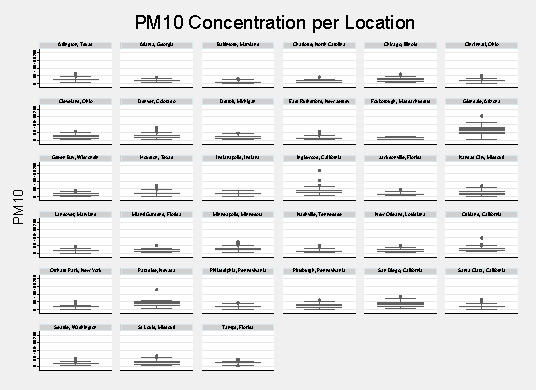
\includegraphics[scale=1.7]{../05_Figures/PM10_Concentration_per_Place.pdf}
	\caption{Box Plot of PM10 Concentration per Location}
	\addvspace{-0.6\baselineskip}
	\caption*{\footnotesize \textit{Source: Own Visualization based on EPA Data.}}
	\label{AppF:1}
\end{figure}
\clearpage
\section{Empirical Framework}
To investigate a potential causal linkage between air pollution and quarterbacks' performances, this term-paper utilizes an empirical framework effectively capturing both unobserved and observed heterogeneity. As visible in the following equation,
\begin{equation}
\hat{Y}_{ijks} = PM10 \times Stadiontype \times \beta + {W'} \zeta + \alpha_i + \mu_{js} + \eta_{ks} + \varepsilon_{ijks},
\end{equation}
the dependent measurement of performance ($\hat{Y}$) is segmented into four dimensions (i.e. i,j,k and s). This four-dimensional segmentation allows to remove time-invariant heterogeneity (i.e. $ \mu_{js} \wedge \eta_{ks}$) as well as individual-specific variation constant over time (i.e. $\alpha_i$). This already reveals that, $i \in Q$ (set of all quarterbacks), $\{s \in \mathbb{Z} \, | \, 2010 \leq s \leq 2022\}$, $j \in T$ (set of teams) and $k \in O$ (set of opponents). Exemplifying the concept, $\hat{Y}_{ijks}$ encapsulates the estimated performance of a quarterback ($i$) within a designated team ($j$), operating against a distinct defensive unit ($k$) during a specified season ($s$).

Consequently, $\mu_{js}$ is the vector of team (offense) by season and $\eta_{ks}$ the vector of opponent (defense) by season fixed effects. Notably, within the NFL, a significant portion of variation can be attributed to changes on a season basis, including transitions like alterations in offensive and defensive coordinators, playbook changes, player acquisitions, and related dynamics. Furthermore, the strategic practice of teams 'tanking' in specific seasons to gain advantageous draft positions highlights the necessity of employing the previously mentioned fixed effects to comprehensively address the diverse but unobserved factors impacting team's and, hence, quarterback's performance. In light of these considerations, additionally including the quarterback-specific effect\footnote{In a pre-check, I do not find any evidence w.r.t. to a season by quarterback variation, which is not already captured in $\mu_{js}$. The same holds for any age variation as deployed by \citet{heintz2022}.}, which encompasses general playstyle, leads to a robust identification framework that effectively accounts for nearly all non-random variation in performance. In spite of this, it's crucial to recognize that while this model covers a wide range of unobserved factors, it doesn't preclude the presence of additional effects on specific game days, e.g. minor injuries. These effects might be considered random draws from a function f($\theta$) with the same probability for all observed performances and being orthogonal to the primary marginal effect of interest. Hence, it can be considered non-influential w.r.t. the causal inference, as it just leads to more noise not affecting the primary effect.\footnote{Generally, this is a strong assumption to make. However, any correlation between $\varepsilon_{ijks}$ and $\Delta PM10$ seems highly unlikely given the data.} The model's setup is completed with ${W'}$, the matrix weather controls by stadiontype, encompassing temperature and precipitation.
\clearpage
\section{Results and Discussion}
\clearpage
\section{Summary and Concluding Remarks}
\clearpage


%------------------------------------------------------------------%
% 4. References
% Insert your .bib name here, then it will automatically generate
% Just cite the papers by \citep{}, \citet{} or \citealp{}
%------------------------------------------------------------------%
\pagenumbering{roman}
\setcounter{page}{\thesavepage}
\pagestyle{plain}
\addcontentsline{toc}{section}{References}
\bibliographystyle{apalike}
\bibliography{EnvEcon.bib}
\clearpage

%------------------------------------------------------------------%
% 5. Appendix
%------------------------------------------------------------------%
\appendix
\section{Further Figures}
\begin{figure}[h]
	\center
	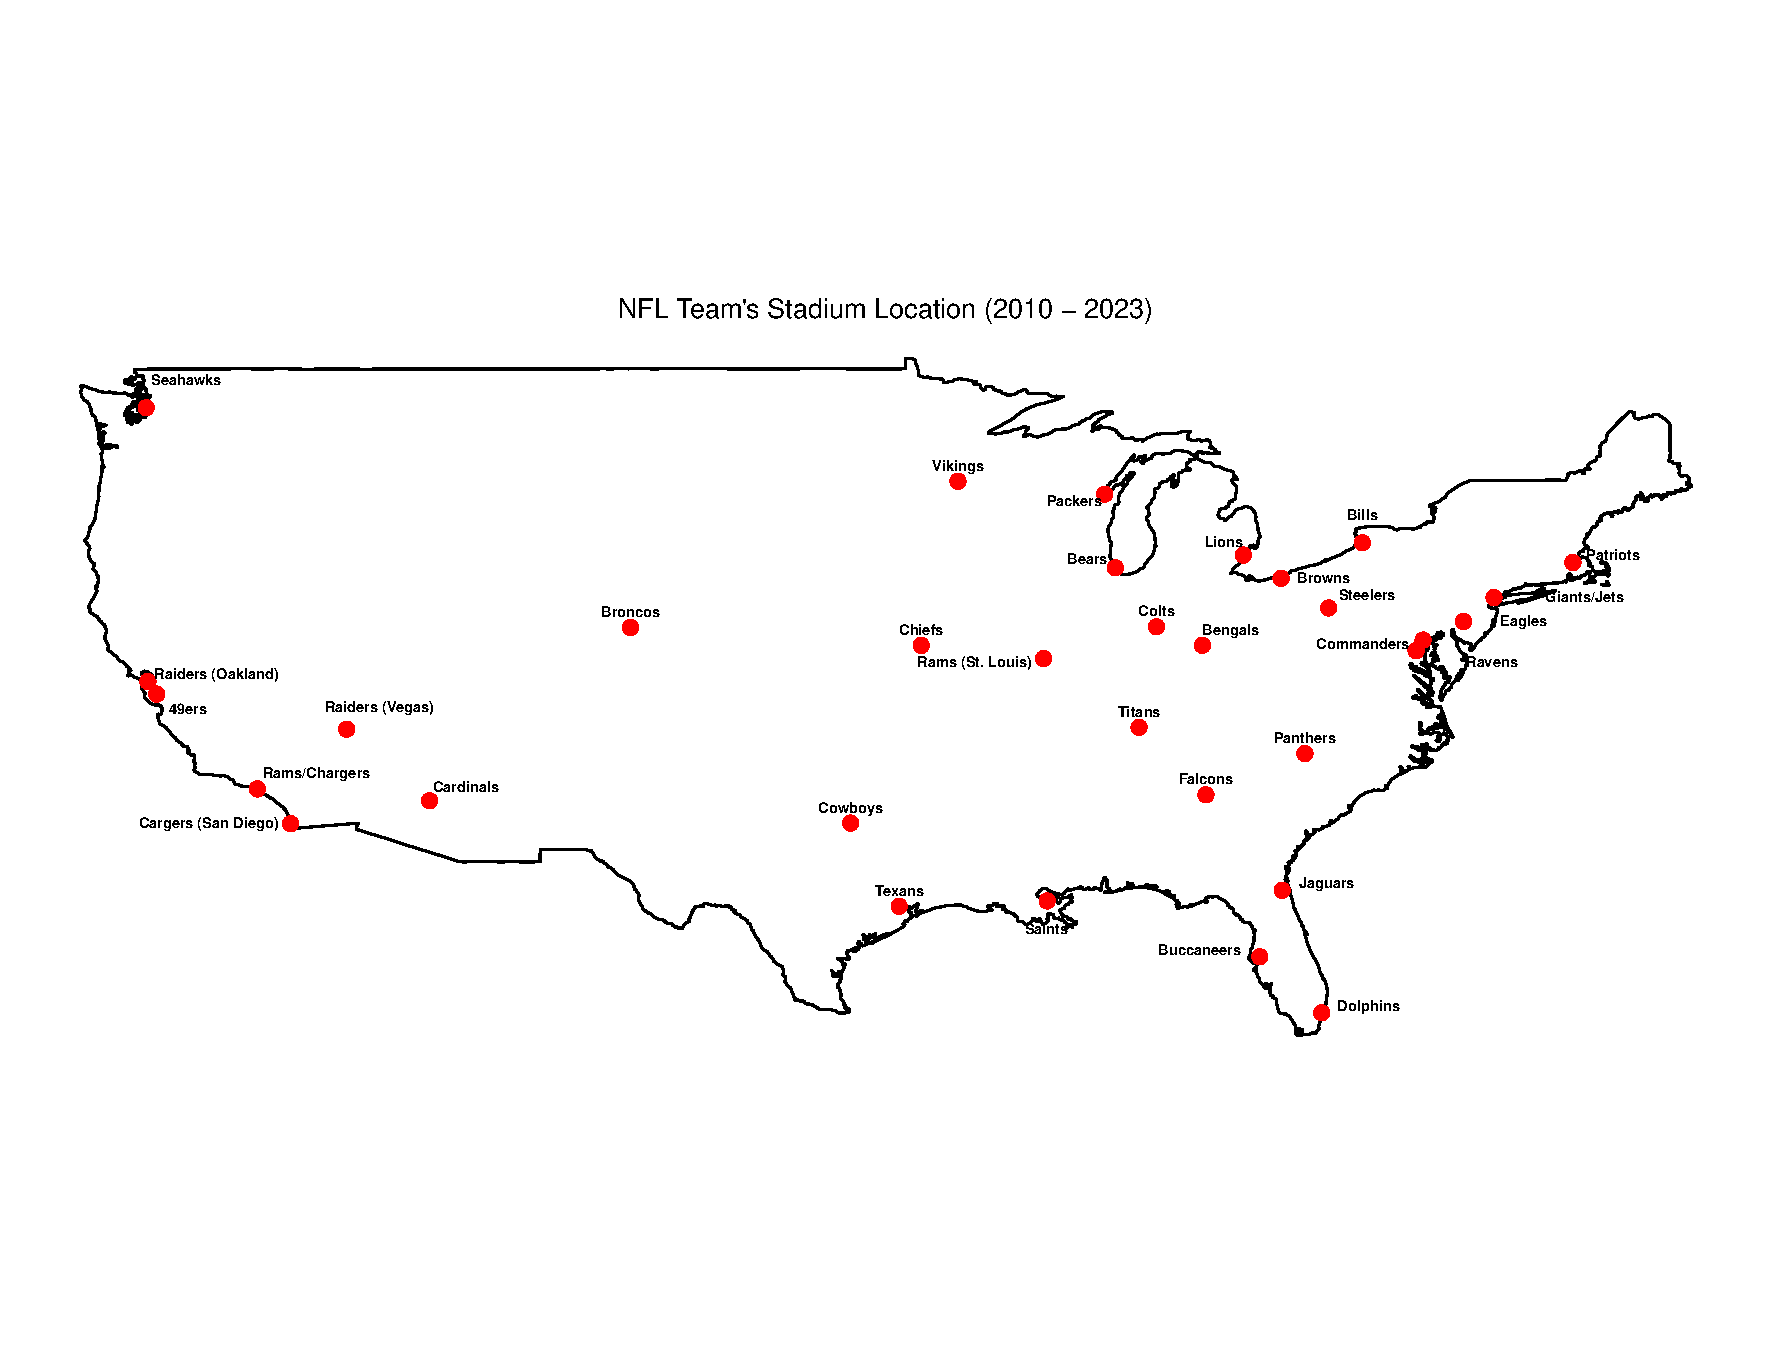
\includegraphics[scale=0.58, angle = 90]{../05_Figures/Teams_Location.pdf}
	\caption{Map of NFL Team's Stadion Locations in Sample}
	\addvspace{-0.6\baselineskip}
	\caption*{\footnotesize \textit{Source: Own Visualization.}}
	\label{F:1}
\end{figure}
\clearpage
\section{Further Tables}


\end{document}
